\section{Benchmarks}
We briefly discuss how we designed the benchmark datasets and corresponding workload.

\subsection{Datasets}
From publicly available sources, we constructed datasets to simulate many envisioned use cases of \textsf{DeepLens}. An important consideration was images of varying format and size. Most academic benchmarks in the machine learning community consist of ``natural images'' in the same format and resolution. We decided that it was important to evaluate a diversity of tasks and the robustness of the injestion pipeline to different formats, sizes, and content. 

\vspace{0.25em} \noindent \textbf{PC.} This dataset is designed to simulate a dataset of images found on a personal computer. It consists of 779 photographs, screenshots, and document scans. 

\vspace{0.25em} \noindent \textbf{TrafficCam.} This dataset consists of 24 mins and 30 secs of high-definition (1080p) traffic camera video. 

\vspace{0.25em} \noindent \textbf{Football.} This dataset consists of 15 low-definition (720p) videos of American football clips of the same team ranging from 30 secs to 1 mins. 

\subsection{Queries}
We propose a benchmark workload of 6 queries on these datasets to evaluate \textsf{DeepLens}. These queries are inspired by problems considered in prior work and consist of task that involve querying pixel data, the results of neural network predictions, relating results back to base data, and combinations.

\vspace{0.25em} \noindent \textbf{q1.} \emph{Find all near-duplicates in the PC dataset}. This query is inspired by classical multimedia information retrieval problems such as reverse image search (find the closest image to a query image). 

\vspace{0.25em} \noindent \textbf{q2.} \emph{Count all of the frames with at least one vehicle present in the TrafficCam dataset}. This query is inspired by recent work that uses neural networks to analyze traffic and movement patterns~\cite{kang2017noscope}. This is a simple query that takes the output of a neural network that identifies objects in the frame and simply queries the output.

\vspace{0.25em} \noindent \textbf{q3.} \emph{Track one player's trajectory in every play in the Football dataset}. Given segmentation output that identifies a player in frame and OCR output that identifies a number if one is visible, we have to relate that sequence of bounding boxes back to the original image.

\vspace{0.25em} \noindent \textbf{q4.} \emph{Count all distinct pedestrians in the TrafficCam dataset}. This query is a variant of q2. The distinct qualifier makes this query significantly more challenging as it requires deduplicating candidate pedestrians detected in the video.

\vspace{0.25em} \noindent \textbf{q5.} \emph{Lookup the presence of a string in the PC dataset}. Apply OCR to all of the images, and store a collection of strings discovered. We run a query to identify the first image with a target string.

\vspace{0.25em} \noindent \textbf{q6.} \emph{Find all tuples of pedestrians (p1,p2) where p1 is behind p2 in the TrafficCam dataset}. This query is inspired from applications in robotics and navigation, where one has to estimate how far a given object is located from a camera. This problem, called depth prediction, has recently been a subject of research interest in computer vision~\cite{depthPredictModel}. We leverage the published code~\footnote{https://github.com/iro-cp/FCRN-DepthPrediction} and the pre-trained parameters to annotate all detected pedestrians in the TrafficCam dataset with depth predictions and find such pairs.

\section{Experiments}
Recent work on video and image analytics systems has largely focused on optimizing neural network inference.
For queries that are simply filters or aggregates, neural network inference clearly dominates the processing cost.
\emph{We use our benchmark to understand the execution profiles of more complex queries.}


\begin{figure}[t]
% \vspace{-5pt}
\centering
 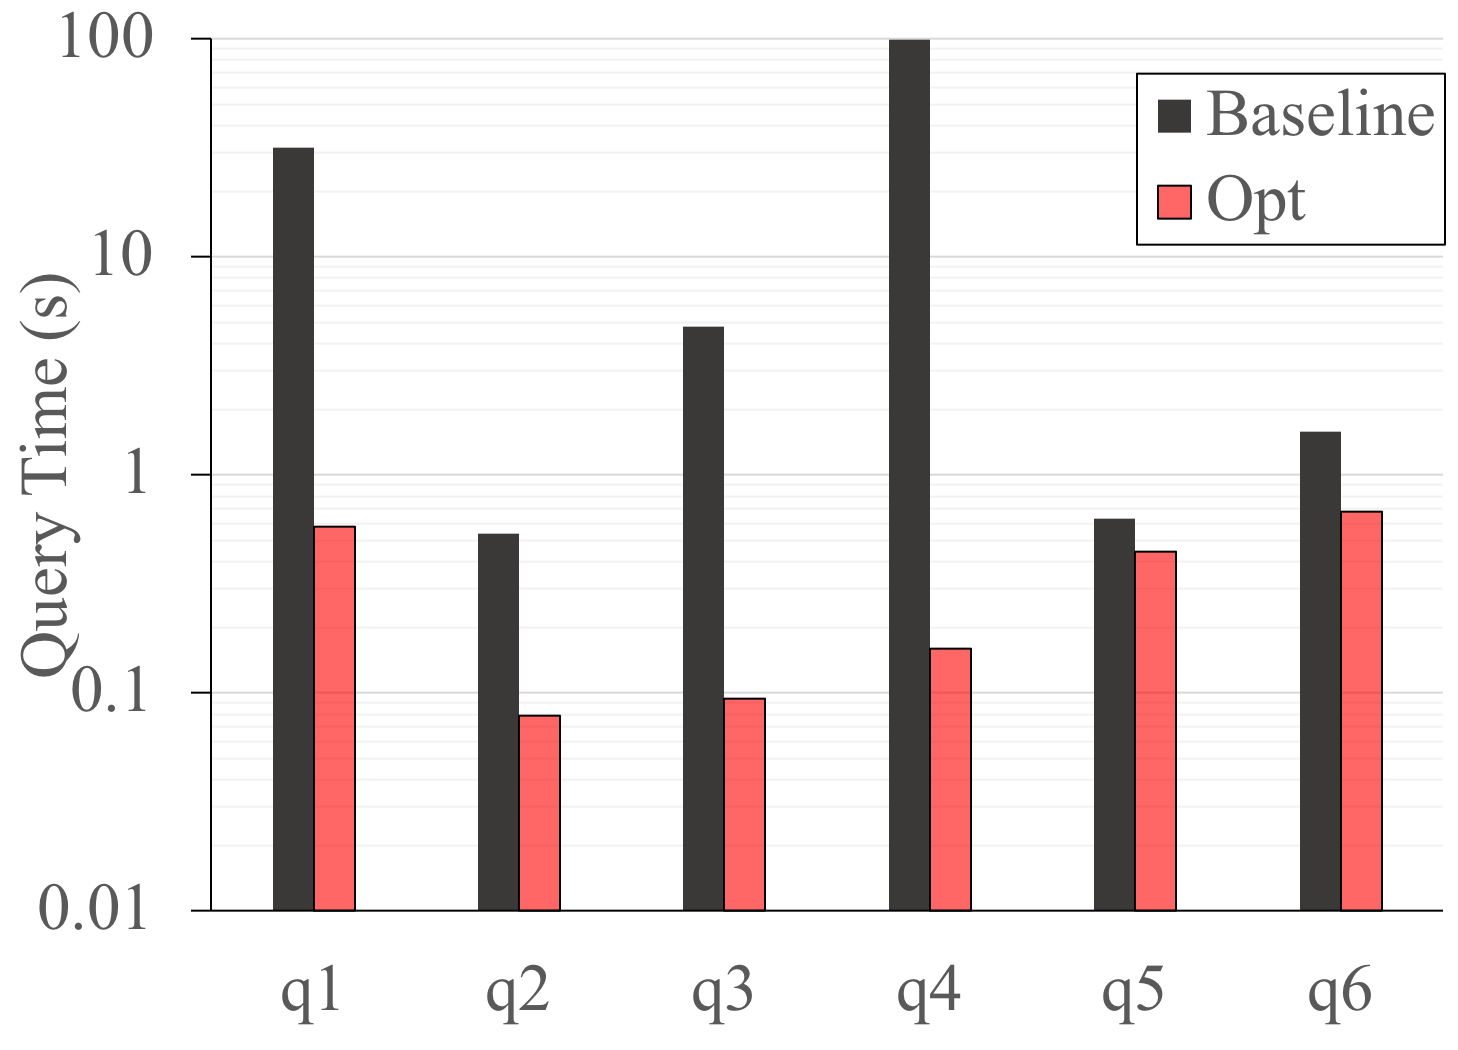
\includegraphics[width=0.8\columnwidth]{figures/query.png}
 \caption{\textsf{DeepLens} significantly speeds up ``query time'' by using indexes. The queries that match multidimensional features can be sped up by up-to 600x.  \label{query} }
\end{figure}

\subsection{The Power of Indexes}
To do so, we separate ``Query time'' (processing results from a neural network) from ``ETL time'' (neural network inference). 
Indexes directly address the problem of query time.
Figure \ref{query} plots the query times with and without indexing.
Our baseline is the same query processing engine with no indexes.
We compare this baseline to a hand-tuned version where we manually select the best physical design for a query.

The queries that benefit the most from the indexes are ones that require image matching, up-to 612x faster for q4 and 59x faster for q1. Note that these matching costs are incurred after neural network inference, so techniques such as~\cite{kang2017noscope, anderson2018predicate, kang2018blazeit} would have no effect on this step.
Queries that have to relate results back to the base images also see improvements since they can leverage the lineage information and do not need to rescan the base data.
q3 requires a backtracing query to match the bounding boxes and the OCR output in pixels on the original image and has a 41x improvement. Similarly, q6 runs 2.5x faster. q5 is illustrative of a query whose predicate does not benefit from any of the available indexes.


\begin{figure}[t]
% \vspace{-5pt}
\centering
 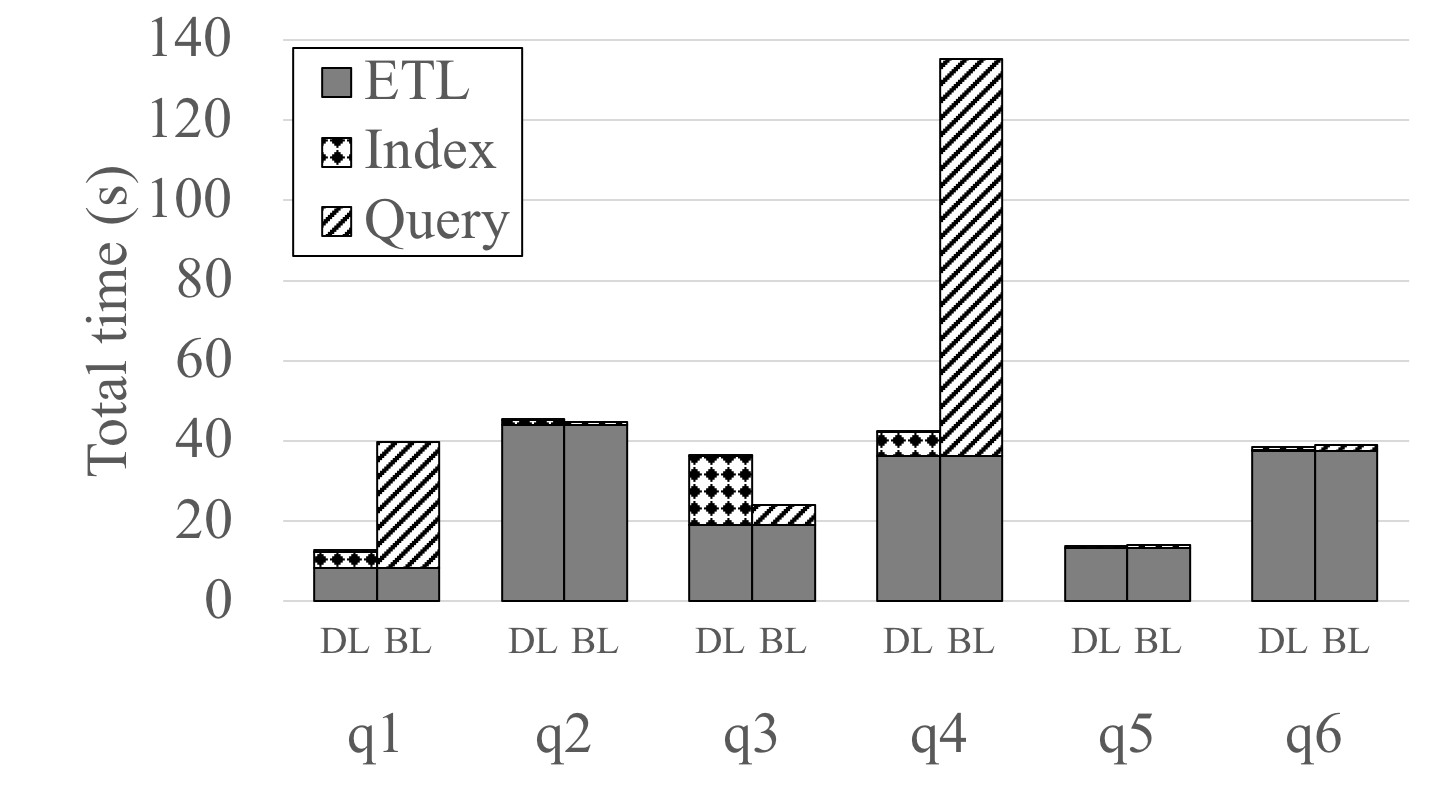
\includegraphics[width=\columnwidth]{figures/indexing_ab.png}
 \caption{We evaluate the pipeline runtime, including ETL and "on-the-fly" index creation, for an optimized \textsf{DeepLens} (DL) vs. the baseline (BL). On many queries it is beneficial to materialize intermediate results and build indexes to speed up future performance. Indexing has a relatively small overhead given the compute-intensive nature of the queries.  \label{index} }
\end{figure}

\begin{figure}[t]
% \vspace{-5pt}
\centering
 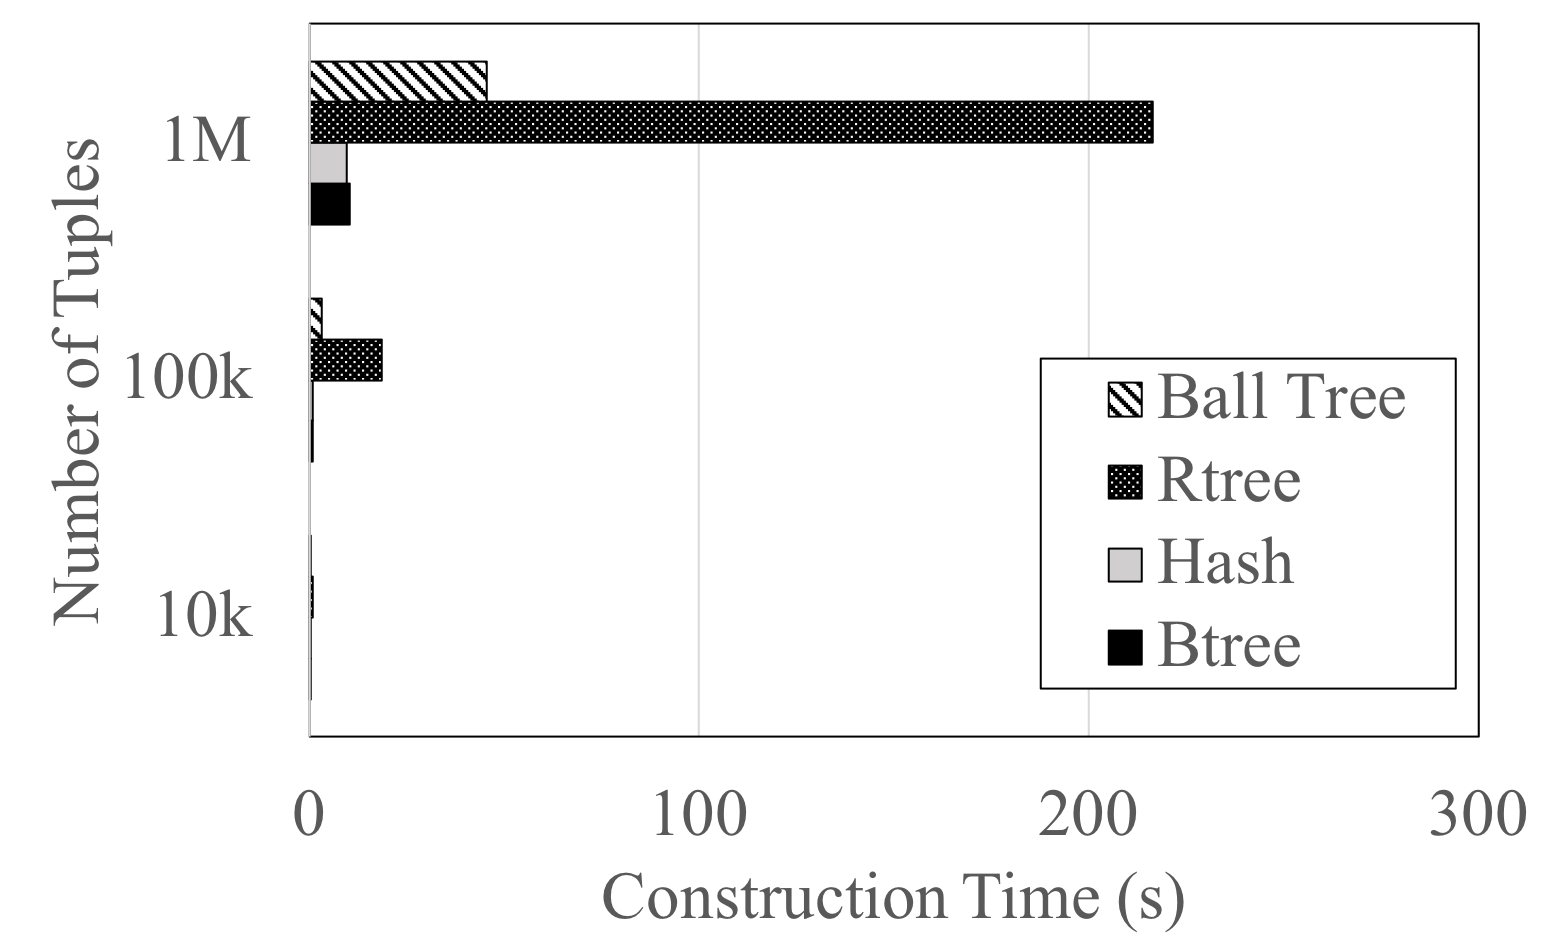
\includegraphics[width=0.8\columnwidth]{figures/indexing.png}
 \caption{Building multidimensional indexes can be very costly and initial experiments indicate that construction time scales poorly with data. \label{indexbuild} }
\end{figure}

\subsection{Overhead For Indexing}
Existing systems in this domain do not make a distinction between Query time and ETL time.
We believe this separation is justified because indexes can be reused by other queries and their construction costs amortize.
Regardless, several of the queries execute faster even if the indexes are built ``on-the-fly'' (Figure \ref{index}).
For example, q1 executes nearly 5 times faster than the baseline and q4 executes 3.5 times faster than the baseline.
The index significantly reduces the number of image matching operations that dominate the runtime, and thus, the cost of building and persisting the index is offset.

The indexes with largest overhead to build are the spatial indexes.
Figure \ref{indexbuild} plots the construction time of the multidimensional and single dimensional indexes supported in \textsf{DeepLens} as a function of the number of tuples indexed.
The R-Tree is nearly 20x slower to construct than a B+ Tree.
However, there are some mitigating factors that are interesting to consider in future work.
Since visual analytics is approximate by nature, perhaps exact multidimensional indexing is unnecessary. 
For some workloads may suffice to apply single dimensional indices and merge results with independence assumptions.
For others, locality sensitive hashing or similar approximations may suffice.

\begin{figure}[t]
% \vspace{-5pt}
\centering
 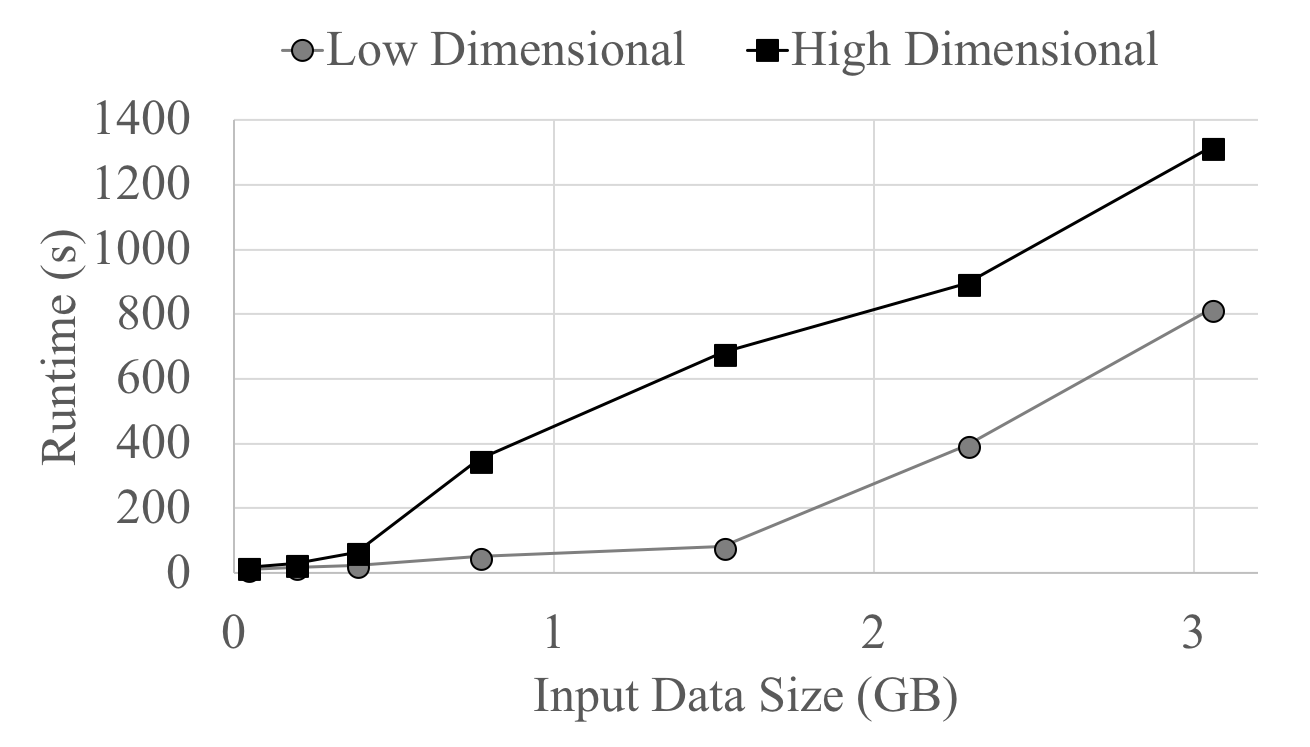
\includegraphics[width=0.8\columnwidth]{figures/spatialjoin.png}
 \caption{We evaluate the execution time of a Ball-Tree join as function of the size of the indexed relation in the high-dimensional and low-dimensional case. As the data structure is increasingly filled the execution time grows non-linearly. \label{join} }
\end{figure}


\subsection{Subtleties in Query Optimization}
For queries that join multiple image collections, neural network inference time does not necessarily dominate.
Optimizing these spatial joins turned out to be more challenging than we thought.

\subsubsection{Nonlinear join costs}
To avoid a large library of hand-written rules, the natural question to ask is whether it is possible to build a cost-based query optimizer for this system.
Figure \ref{join} illustrates the difficulties with the execution time of a Ball-Tree join as function of the size of the indexed relation in the high-dimensional and low-dimensional case. As the data structure is increasingly filled the execution time grows non-linearly. The non-linearity is also data-dependent and is more extreme in higher dimensional data. Accurately modeling the relationship between input relation size and operator cost is crucical for cost-based query optimization. Non-linearities are also known to affect standard join ordering heuristics~\cite{krishnan2018deeprljoins}.

\subsubsection{Balancing CPU vs. GPU}
Processing these complex queries requires a nuanced strategy in balancing CPU vs. GPU usage. 
For the ETL phase of these queries, which is dominated by neural network inference time, using the GPU is almost universally better.
Figure \ref{build} (left) plots the processing time on each of the six benchmark queries for a vanilla CPU implementation (CPU), a vectorized execution (AVX), and a GPU implementation (GPU). Just by changing the underlying execution architecture there were up-to 12x changes in execution time. 
On the other hand, the results were more mixed for the query time. 
For the two image matching queries, q1 and q4, we implemented an all pairs matching comparison with vectorization and on the GPU.
For the larger query (q4) there is a significant performance benefit from using the GPU (34\% faster).
For the smaller query (q1), the overhead of using the GPU outweighs the costs.
Any cost-based optimizer has to weigh overheads before selecting a plan.


\begin{figure}[t]
% \vspace{-5pt}
\centering
 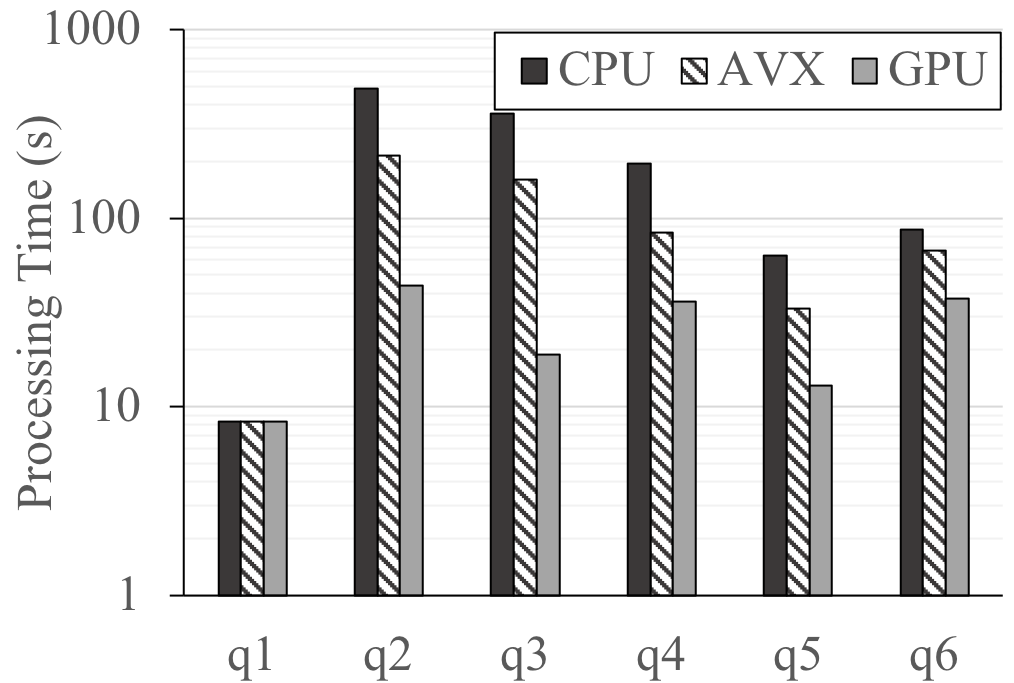
\includegraphics[width=0.48\columnwidth]{figures/build.png}
  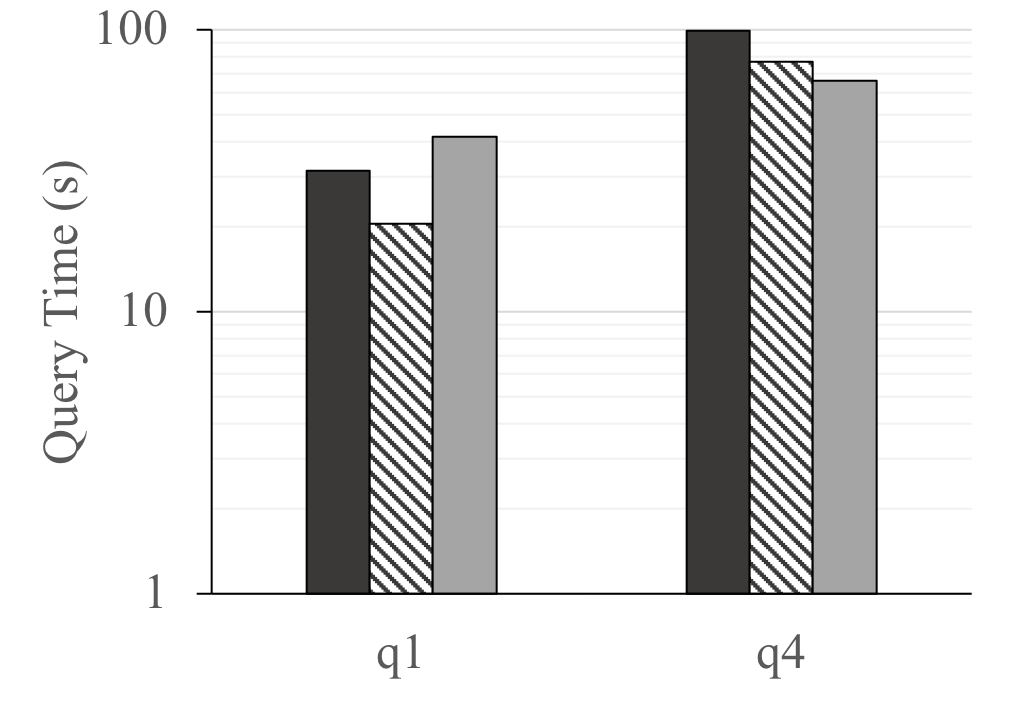
\includegraphics[width=0.48\columnwidth]{figures/build2.png}
 \caption{The execution architecture has a considerable impact on both ETL and Query time: vanilla CPU implementation (CPU), a vectorized execution (AVX), and GPU implementation (GPU). GPUs are significantly more efficient for the neural network dominated ETL time, but have more mixed results for the subsequent query processing on two image matching queries (q1, q4).  \label{build} }
\end{figure}

\subsubsection{Accuracy implications of different query plans}
Unlike in relational databases, queries in a VDMS are approximate by nature.
Cascades of approximate operators can have correlations in their errors that are hard to reason about.
These errors can be affected by query optimizer choices.
Let us take q4 as an example.
To process this query, the system first identifies patches using an object detector, then filters those patches to those that are people, and then matches all pairs of patches to deduplicate.
In another approach, the system would first identify patches using an object detector, then match all pairs of patches (regardless if they are ``people'') to deduplicate, and finally filter on those pairs that have at least one person label.
The second approach goes against typical query optimization principles of filter pushdown--but we see that it is actually a more accurate strategy.

\begin{table}[]
\centering
\begin{tabular}{|c|c|c|c|}
\hline
Execution method for q4 & Recall               & Precision & Runtime         \\
\hline
Patch, Filter, Match & 0.73      & 0.97    & 34.56  \\
Patch, Match, Filter & 0.82      & 0.98    & 62.11  \\
\hline
\end{tabular}
\caption{Accuracy vs. runtime for different execution methods query of q4.} \label{tab:q4execution}
\end{table}


